\section{Stellarmate}

\subsection{Paramount}
This page helps with installation for Paramount:
https://www.indilib.org/devices/mounts/bisque-paramount.html

\begin{figure}[h!]
\centering
\begingroup \fontsize{10pt}{10pt}
\selectfont
\begin{verbatim} 
# if using a Paramount
apt-add-repository ppa:mutlaqja/ppa
apt-get update 
sudo apt-get install libindi

cat >> /home/stellarmate/help.txt <<EOF
Paramount: In TheSkyX preferences, make sure to turn off TCP Responses close socket.
EOF
\end{verbatim}
\endgroup
\caption{Raspberry Pi, Paramount packages to install.}
\label{figure:RaspberryPiParamount}
\end{figure}

Stellarmate uses the TCP connection for the mount. Needs port address of the mount's
PC.


From \url{https://www.indilib.org/devices/mounts/bisque-paramount.html}

\begin{figure}[h!]
\centering
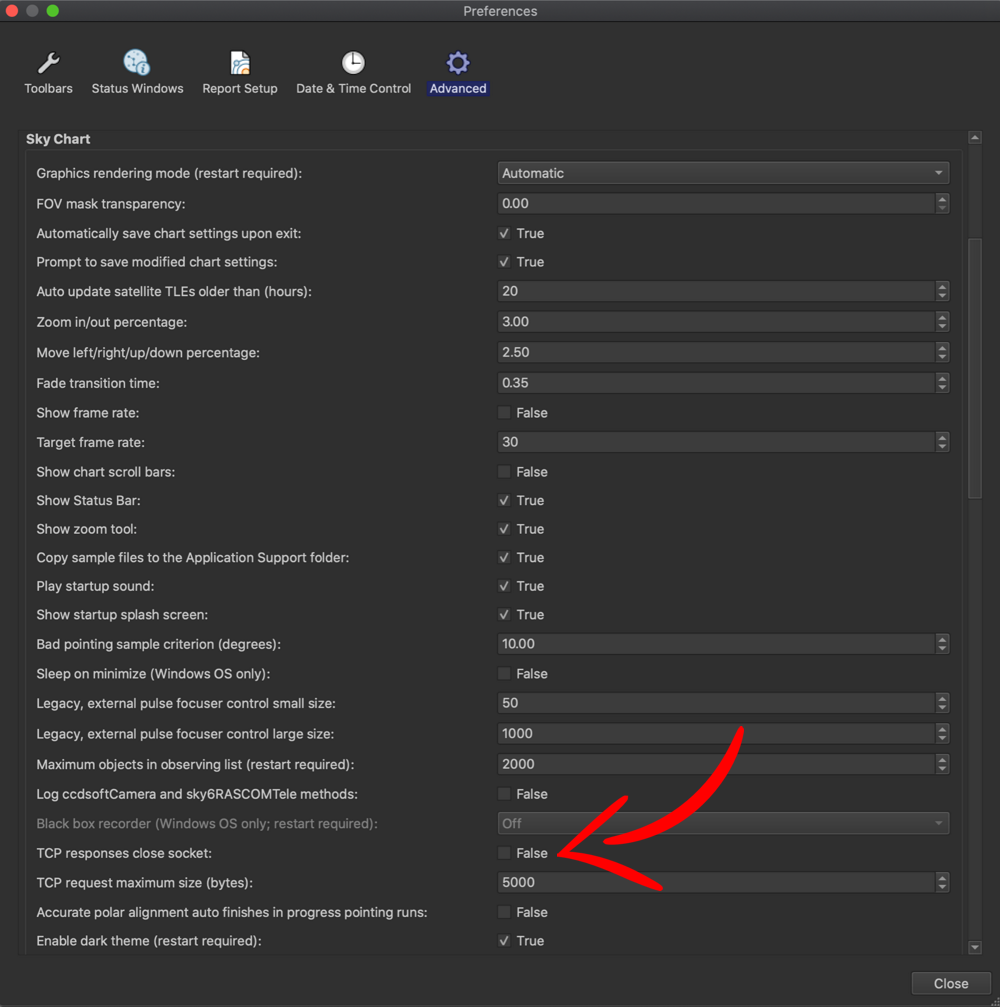
\includegraphics[width=\textwidth]{images/smate_theskyx_config.png}
\caption[TheSkyX preferences]{In TheSkyX preferences, make sure to turn off TCP Responses close socket}
\label{figure:SmateTheskyxConfig}
\end{figure}

\begin{figure}[h!]
\centering
\includegraphics[width=\textwidth]{images/smate_paramount_options-2.png}
\caption[Stellarmate paramount options]{Fill in the telescope parameters, and set
up to record to a log file.}
\label{figure:SmateParamountOptions }
\end{figure}

\begin{figure}[h!]
\centering
\includegraphics[width=\textwidth]{images/smate_paramount_connection-2.png}
\caption[Stellarmate paramount connection]{Stellarmate paramount connection, this is
the IP address of the Sky X Computer, default port (3040) for TCP control.}
\label{figure:SmateParamountConnection.png}
es
\end{figure}

